\textbf{Tracking points using Lucas-Kanade method}

I have used Lucas Kanade's method to track the points in the video. The points that are to be tracked are resolved by \textit{cv2.goodFeaturesToTrack()} function. The points are then tracked. The points are then visualized using trailing lines to indicate the motion of point.

\begin{figure}[H]
    \centering
    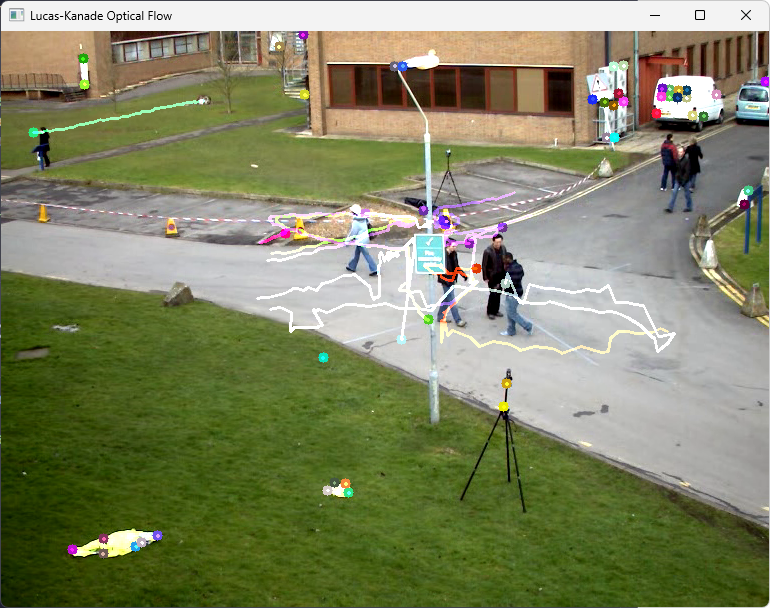
\includegraphics[width=1\textwidth]{res/lk_track.png}
    \caption{Optical flow}
    \label{fig:2.1}
\end{figure}

\newpage

\textbf{Visualization through arrows}

The direction of the motion is visualized using arrows. The arrows are drawn from the point to the direction of the motion. The length of the arrow is proportional to the speed of the motion.

\begin{figure}[H]
    \centering
    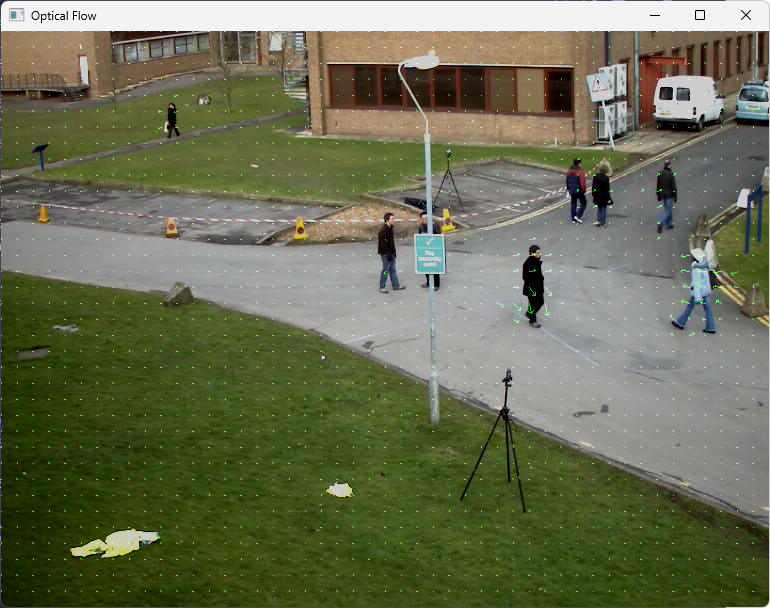
\includegraphics[width=1\textwidth]{res/optical_flow.png}
    \caption{Optical flow with arrows}
    \label{fig:2.2}
\end{figure}

\textbf{Summary}

The movement of pedestrian is composed of mostly straight lines. The pedestrians tend to cluster at the center of the crosswalk, at the branching. The pedestrians tend to move faster in the center of the crosswalk. The pedestrians tend to move slower at the edges of the crosswalk. This can be observed in the image attached above. The pedestrians tend to move in the direction of the road.